\documentclass[11pt]{article}

\usepackage[margin=1in]{geometry}
\usepackage{amsmath,amssymb,amsthm,mathtools}
\usepackage{tikz}
\usetikzlibrary{calc}
\usepackage{hyperref}
\usepackage{enumitem}

\title{Modeling the Cart--Pole Inverted Pendulum:\\
Lagrangian Dynamics, Linearization, and LQR Control}
\author{Ethan Lemke}
\date{\today}

% --- a lightweight "tangent" environment built only from core LaTeX,
% so this compiles anywhere without extra packages ---
\newenvironment{tangent}[1]{%
  \par\smallskip\noindent\hrulefill\par
  \noindent\textbf{Tangent — #1.}\par\smallskip
  \begingroup\itshape
}{%
  \endgroup
  \par\noindent\hrulefill\par\smallskip
}

\newcommand{\mb}[1]{\mathbf{#1}}

\begin{document}
\maketitle

\begin{abstract}
This document derives, from first principles, the full nonlinear dynamics of
the cart--pole (inverted pendulum) balancer, linearizes them about the
upright equilibrium, proves controllability, and derives the LQR balancing
controller from the underlying optimal-control theory. It corresponds to
Phase 3 (\emph{Understand and model the physics}) and Phase 4
(\emph{Design the balance controller}) of the project roadmap. Phase 5
(energy-based swing-up) and Phase 6 (polish/robustness) are intentionally
out of scope here and will be treated in a later document. Numeric physical
parameters (pendulum mass/length, cart mass, friction coefficients, travel
limits) have not yet been measured on the hardware; every result below is
therefore left symbolic so that measured values can simply be substituted
in once available.
\end{abstract}

\tableofcontents

\part{Physics Modeling (Phase 3)}

\section{System Description and Notation}

The physical system is a motorized carriage that translates horizontally
along a linear rail (belt-driven by a NEMA17 stepper through a TMC2209
driver), with a rigid steel rod pendulum pivoted to the carriage through an
LPD3806 rotary encoder. The encoder measures the pendulum's angle relative
to the carriage; the stepper effectively lets us command a horizontal force
(or, at the step-command level, a position/velocity) on the carriage.

\subsection{Modeling assumptions}
\begin{itemize}[leftmargin=*]
  \item Planar motion only (no out-of-rail-plane dynamics).
  \item The rail is horizontal and rigid; the carriage moves without
    vertical motion.
  \item The pendulum is a \emph{rigid, uniform rod} — not a point mass. Its
    rotational inertia about its own center of mass matters and is carried
    through the derivation explicitly (this is what makes the model a
    \emph{physical} pendulum rather than the simplified \emph{simple}
    pendulum many textbook treatments use).
  \item Belt/drivetrain dynamics (stepper torque ripple, belt compliance,
    backlash, discretized step motion) are abstracted away: we model the
    actuator as producing an ideal continuous horizontal force $u$ directly
    on the carriage. This is a real modeling gap to revisit during Phase 6
    (robustness) once the idealized controller is working; it is standard
    practice to idealize the actuator first and treat its non-idealities as
    disturbances/uncertainty to be handled by controller robustness margin
    and empirical tuning, rather than modeled analytically up front.
  \item Friction is modeled as simple viscous (linear-in-velocity) damping
    at the carriage/rail interface and at the pivot bearing. Coulomb
    (static/kinetic) friction and any pivot backlash are neglected for now.
\end{itemize}

\subsection{Coordinates and parameters}

\begin{center}
\begin{tabular}{p{0.32\textwidth}p{0.6\textwidth}}
\hline
Symbol & Meaning \\
\hline
$x$ & Carriage (cart) position along the rail [m] \\
$\theta$ & Pendulum angle, measured from the \emph{upward} vertical,
  positive in the $+x$ tilt direction [rad] \\
$m_c$ & Carriage mass [kg] \\
$m_p$ & Pendulum (rod) mass [kg] \\
$L$ & Full rod length [m] \\
$\ell_c = L/2$ & Distance from pivot to rod center of mass (uniform rod)
  [m] \\
$I_{\mathrm{cm}} = \tfrac{1}{12} m_p L^2$ & Rod's moment of inertia about
  its own center of mass \\
$I_p = I_{\mathrm{cm}} + m_p \ell_c^2 = \tfrac{1}{3} m_p L^2$ & Rod's
  moment of inertia about the pivot (see \S\ref{sec:parallelaxis}) \\
$g$ & Gravitational acceleration [m/s$^2$] \\
$b_x$ & Viscous friction coefficient, carriage/rail [N$\cdot$s/m] \\
$b_\theta$ & Viscous friction coefficient, pivot bearing
  [N$\cdot$m$\cdot$s/rad] \\
$u$ & Control input: horizontal force applied to the carriage [N] \\
\hline
\end{tabular}
\end{center}

\begin{quote}
\textbf{Notation collision, flagged up front:} controls literature
universally writes the \emph{state vector} in bold as $\mb x =
[x,\dot x,\theta,\dot\theta]^\top$, while the very same letter $x$ (not
bold) is the cart's position — one of the four entries of $\mb x$. Both
conventions are too standard to abandon, so both are kept; bold vs.\ not
bold disambiguates throughout.
\end{quote}

Figure~\ref{fig:cartpole} shows the sign convention: $\theta = 0$ is
straight up (the unstable equilibrium we want to balance at), and positive
$\theta$ tilts the rod toward $+x$.

\begin{figure}[h]
\centering
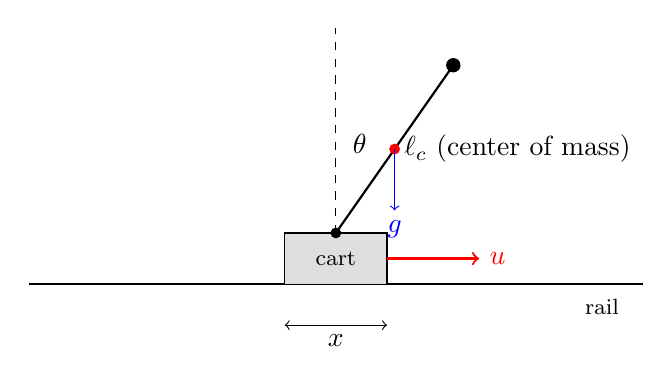
\begin{tikzpicture}[scale=1.3]
  % rail
  \draw[thick] (-3,0) -- (3,0);
  \node[below] at (2.6,-0.05) {\footnotesize rail};
  % cart
  \draw[fill=gray!25] (-0.5,0) rectangle (0.5,0.5);
  \node at (0,0.25) {\footnotesize cart};
  % pivot
  \coordinate (P) at (0,0.5);
  \fill (P) circle (1.5pt);
  % vertical dashed reference
  \draw[dashed] (P) -- ++(0,2);
  % rod, tilted theta from vertical toward +x
  \draw[thick] (P) -- ++(55:2) coordinate (Tip);
  \fill (Tip) circle (2pt);
  % theta label (no precise arc, just illustrative placement)
  \node at ($(P)+(75:0.9)$) {$\theta$};
  % center of mass marker
  \coordinate (CoM) at ($(P)!0.5!(Tip)$);
  \fill[red] (CoM) circle (1.5pt);
  \node[right] at (CoM) {$\ell_c$ (center of mass)};
  % gravity arrow
  \draw[->,blue] (CoM) -- ++(0,-0.6) node[below]{$g$};
  % control force arrow
  \draw[->,thick,red] (0.5,0.25) -- ++(0.9,0) node[right]{$u$};
  % x span
  \draw[<->] (-0.5,-0.4) -- (0.5,-0.4);
  \node[below] at (0,-0.4) {$x$};
\end{tikzpicture}
\caption{Cart--pole sign convention. $\theta$ measured from upward
vertical; $u$ is the horizontal actuator force on the cart.}
\label{fig:cartpole}
\end{figure}

\begin{tangent}{the parallel axis theorem}
\label{sec:parallelaxis}
For a rigid body of mass $m$, the moment of inertia about \emph{any} axis
parallel to one through the center of mass is
\[
  I_{\text{axis}} = I_{\mathrm{cm}} + m d^2,
\]
where $d$ is the distance between the two parallel axes. This follows
directly from expanding $I_{\text{axis}} = \int \|\mb r - \mb r_{\text{axis}}\|^2\, dm$
in terms of the center-of-mass position and using $\int (\mb r - \mb
r_{\mathrm{cm}})\,dm = 0$ by definition of the center of mass — the cross
term vanishes, leaving exactly $I_{\mathrm{cm}} + md^2$. For a uniform rod
of length $L$ pivoted at one end, $d = \ell_c = L/2$ and $I_{\mathrm{cm}} =
\tfrac{1}{12}mL^2$, giving the familiar $I_p = \tfrac{1}{12}mL^2 +
m(L/2)^2 = \tfrac{1}{3}mL^2$.
\end{tangent}

\section{Lagrangian Mechanics Primer}

\begin{tangent}{why Lagrangian mechanics instead of Newton--Euler here}
Newton--Euler mechanics requires drawing every free body (cart, rod),
introducing the unknown constraint/reaction forces at the pivot and rail
(normal forces, pivot pin reactions), writing $F=ma$ and $\tau = I\alpha$
for each body, and then algebraically eliminating the reaction forces to
get back down to two equations in $x,\theta$. Lagrangian mechanics reaches
the same two equations directly, because the reaction/constraint forces of
an \emph{ideal} constraint (rigid rod, frictionless-in-the-constraint-
direction rail) do zero virtual work and simply never appear. For a
two-body, two-constrained-DOF system like this one, that is a substantial
simplification.
\end{tangent}

\begin{tangent}{generalized coordinates, Hamilton's principle, and the
Euler--Lagrange equation}
A \emph{generalized coordinate} set $q_1,\dots,q_n$ is any minimal set of
parameters that fully determines the configuration of the system — here
$n=2$, $q = (x,\theta)$, since fixing $x$ and $\theta$ fixes the position
of every point of the cart and rod. Define the Lagrangian $\mathcal L(q,
\dot q) = T(q,\dot q) - V(q)$, kinetic minus potential energy, and the
action functional over a candidate trajectory $q(t)$ on $[t_0,t_1]$ with
fixed endpoints:
\[
  S[q] = \int_{t_0}^{t_1} \mathcal L(q(t),\dot q(t))\,dt.
\]
\emph{Hamilton's principle} states that the true trajectory of the system
is a stationary point of $S$: $\delta S = 0$ for all admissible variations
$\delta q(t)$ vanishing at the endpoints. Writing $q \to q+\epsilon\eta$
for a smooth perturbation $\eta$ with $\eta(t_0)=\eta(t_1)=0$, and
differentiating $S$ with respect to $\epsilon$ at $\epsilon=0$:
\[
  0 = \frac{d}{d\epsilon}\Big|_{0} S[q+\epsilon\eta]
    = \int_{t_0}^{t_1}\left(\frac{\partial \mathcal L}{\partial q}\eta
      + \frac{\partial \mathcal L}{\partial \dot q}\dot\eta\right) dt.
\]
Integrating the second term by parts (the boundary term vanishes because
$\eta(t_0)=\eta(t_1)=0$) gives
$\int \left(\frac{\partial \mathcal L}{\partial q} -
\frac{d}{dt}\frac{\partial \mathcal L}{\partial \dot q}\right)\eta\,dt = 0$
for \emph{every} admissible $\eta$, so by the fundamental lemma of the
calculus of variations the bracketed quantity must vanish identically:
\[
  \frac{d}{dt}\frac{\partial \mathcal L}{\partial \dot q_i}
  - \frac{\partial \mathcal L}{\partial q_i} = 0, \qquad i=1,\dots,n.
\]
This is the \emph{Euler--Lagrange equation}. When non-conservative
(externally applied or dissipative) generalized forces $Q_i$ act on
coordinate $q_i$ — here, the motor force and friction torque/force, which
are \emph{not} derivable from a potential — the same derivation with
virtual work $\sum_i Q_i\,\delta q_i$ added to the variation yields the
more general form actually used below:
\[
  \frac{d}{dt}\frac{\partial \mathcal L}{\partial \dot q_i}
  - \frac{\partial \mathcal L}{\partial q_i} = Q_i.
\]
\end{tangent}

\section{Kinematics}

Take the pivot (top of the carriage) as the reference point. With $\theta$
measured from upward vertical as in Figure~\ref{fig:cartpole}, the pivot
sits at $(x,0)$ and the rod's center of mass sits at
\[
  \mb r_{\mathrm{cm}} = \big(x + \ell_c\sin\theta,\ \ell_c\cos\theta\big).
\]
Differentiating,
\[
  \dot{\mb r}_{\mathrm{cm}} =
  \big(\dot x + \ell_c\cos\theta\,\dot\theta,\ -\ell_c\sin\theta\,\dot\theta\big),
\]
so the squared speed of the center of mass is
\begin{align*}
  v_{\mathrm{cm}}^2 &= (\dot x + \ell_c\cos\theta\,\dot\theta)^2
     + (\ell_c\sin\theta\,\dot\theta)^2 \\
  &= \dot x^2 + 2\ell_c\cos\theta\,\dot x\dot\theta
     + \ell_c^2\cos^2\theta\,\dot\theta^2 + \ell_c^2\sin^2\theta\,\dot\theta^2\\
  &= \dot x^2 + 2\ell_c\cos\theta\,\dot x\dot\theta + \ell_c^2\dot\theta^2,
\end{align*}
using $\sin^2\theta+\cos^2\theta = 1$.

\section{Energy and the Lagrangian}

\subsection{Kinetic energy}
The carriage translates without rotating: $T_{\mathrm{cart}} =
\tfrac12 m_c\dot x^2$. The rod has both translational kinetic energy of
its center of mass and rotational kinetic energy about that center of
mass:
\[
  T_{\mathrm{rod}} = \tfrac12 m_p v_{\mathrm{cm}}^2 + \tfrac12
  I_{\mathrm{cm}}\dot\theta^2.
\]
Summing and substituting $v_{\mathrm{cm}}^2$ from above,
\begin{align}
  T &= \tfrac12 m_c\dot x^2 + \tfrac12 m_p\left(\dot x^2 +
  2\ell_c\cos\theta\,\dot x\dot\theta + \ell_c^2\dot\theta^2\right)
  + \tfrac12 I_{\mathrm{cm}}\dot\theta^2 \notag\\
  &= \tfrac12 (m_c+m_p)\dot x^2 + m_p\ell_c\cos\theta\,\dot x\dot\theta
  + \tfrac12\big(I_{\mathrm{cm}} + m_p\ell_c^2\big)\dot\theta^2 \notag\\
  &= \tfrac12 (m_c+m_p)\dot x^2 + m_p\ell_c\cos\theta\,\dot x\dot\theta
  + \tfrac12 I_p\dot\theta^2, \label{eq:kinetic}
\end{align}
where the last step used $I_p = I_{\mathrm{cm}}+m_p\ell_c^2$ from the
parallel axis theorem (\S\ref{sec:parallelaxis}) to fold the translational
and rotational rod terms into a single moment of inertia about the pivot.

\subsection{Potential energy}
Taking the pivot height as the zero reference,
\begin{equation}
  V = m_p g \ell_c\cos\theta. \label{eq:potential}
\end{equation}
Note $V$ is \emph{maximized} at $\theta=0$ (upright) and minimized at
$\theta=\pi$ (hanging straight down) — consistent with upright being the
unstable, high-potential-energy equilibrium we are trying to balance at,
and hanging-down being the passive, stable, low-energy equilibrium.

\begin{tangent}{total mechanical energy and power balance}
Define $E = T+V$. Differentiating along any trajectory and using the
equations of motion derived in the next section, one finds
$\dot E = u\dot x - b_x\dot x^2 - b_\theta\dot\theta^2$: the actuator
injects power $u\dot x$, and friction dissipates power
$b_x\dot x^2+b_\theta\dot\theta^2 \ge 0$. With $u=0$ and no friction,
$E$ is exactly conserved — a good numerical sanity check for a simulator
(integrate the frictionless, unforced equations and confirm $E$ stays
constant to integrator tolerance). This $E$ is also the quantity a
swing-up controller (Phase 5, deferred) would regulate toward the upright
value $E^\star = m_p g\ell_c$ — noted here for completeness since it falls
straight out of $T$ and $V$, not because swing-up is being designed now.
\end{tangent}

\subsection{The Lagrangian}
\begin{equation}
  \mathcal L = T - V = \tfrac12(m_c+m_p)\dot x^2 + m_p\ell_c\cos\theta\,
  \dot x\dot\theta + \tfrac12 I_p\dot\theta^2 - m_p g\ell_c\cos\theta.
  \label{eq:lagrangian}
\end{equation}

\section{Nonlinear Equations of Motion}

The non-conservative generalized forces are the actuator force (acting on
$x$) and viscous friction (acting on both coordinates, opposing motion):
\[
  Q_x = u - b_x\dot x, \qquad Q_\theta = -b_\theta\dot\theta.
\]

\subsection{The $x$ equation}
From \eqref{eq:lagrangian}, $\dfrac{\partial\mathcal L}{\partial\dot x} =
(m_c+m_p)\dot x + m_p\ell_c\cos\theta\,\dot\theta$ and
$\dfrac{\partial\mathcal L}{\partial x}=0$ ($x$ does not appear
explicitly in $\mathcal L$ — see the cyclic-coordinate remark in
\S\ref{sec:equilibria}). So
\[
  \frac{d}{dt}\frac{\partial\mathcal L}{\partial\dot x} =
  (m_c+m_p)\ddot x + m_p\ell_c\cos\theta\,\ddot\theta
  - m_p\ell_c\sin\theta\,\dot\theta^2,
\]
and the Euler--Lagrange equation
$\frac{d}{dt}\frac{\partial\mathcal L}{\partial\dot x} -
\frac{\partial\mathcal L}{\partial x} = Q_x$ gives
\begin{equation}
  (m_c+m_p)\ddot x + m_p\ell_c\cos\theta\,\ddot\theta
  - m_p\ell_c\sin\theta\,\dot\theta^2 + b_x\dot x = u. \label{eq:eom1}
\end{equation}

\subsection{The $\theta$ equation}
$\dfrac{\partial\mathcal L}{\partial\dot\theta} = m_p\ell_c\cos\theta\,
\dot x + I_p\dot\theta$, so
\[
  \frac{d}{dt}\frac{\partial\mathcal L}{\partial\dot\theta} =
  m_p\ell_c\cos\theta\,\ddot x - m_p\ell_c\sin\theta\,\dot x\dot\theta
  + I_p\ddot\theta.
\]
Also $\dfrac{\partial\mathcal L}{\partial\theta} = -m_p\ell_c\sin\theta\,
\dot x\dot\theta + m_p g\ell_c\sin\theta$ (differentiating the $\cos\theta$
terms in $\mathcal L$). Subtracting,
\[
  \frac{d}{dt}\frac{\partial\mathcal L}{\partial\dot\theta}
  - \frac{\partial\mathcal L}{\partial\theta} =
  m_p\ell_c\cos\theta\,\ddot x + I_p\ddot\theta - m_p g\ell_c\sin\theta,
\]
the $-m_p\ell_c\sin\theta\,\dot x\dot\theta$ Coriolis-type term canceling
exactly between the two pieces. Setting this equal to $Q_\theta$:
\begin{equation}
  I_p\ddot\theta + m_p\ell_c\cos\theta\,\ddot x
  - m_p g\ell_c\sin\theta + b_\theta\dot\theta = 0. \label{eq:eom2}
\end{equation}

Equations \eqref{eq:eom1}--\eqref{eq:eom2} are the full nonlinear cart-pole
dynamics — a coupled pair of second-order ODEs in $x,\theta$, exact (given
the stated modeling assumptions), for any amplitude of $\theta$.

\subsection{Manipulator (mass-matrix) form}
It is standard, and useful for simulation, to write \eqref{eq:eom1}--
\eqref{eq:eom2} as $M(\theta)\ddot{\mb q} + \mb c(\theta,\dot\theta) +
\mb d(\dot{\mb q}) + \mb g(\theta) = \mb B u$, with $\mb q =
(x,\theta)^\top$:
\[
  M(\theta) = \begin{bmatrix} m_c+m_p & m_p\ell_c\cos\theta \\
  m_p\ell_c\cos\theta & I_p \end{bmatrix},\quad
  \mb c = \begin{bmatrix} -m_p\ell_c\sin\theta\,\dot\theta^2 \\ 0
  \end{bmatrix},\quad
  \mb d = \begin{bmatrix} b_x\dot x \\ b_\theta\dot\theta\end{bmatrix},
\]
\[
  \mb g(\theta) = \begin{bmatrix} 0 \\ -m_p g\ell_c\sin\theta
  \end{bmatrix}, \qquad
  \mb B = \begin{bmatrix} 1 \\ 0 \end{bmatrix}.
\]
$M(\theta)$ is symmetric positive definite for all $\theta$ (it is a
kinetic-energy/mass matrix — physically, kinetic energy $T =
\tfrac12\dot{\mb q}^\top M\dot{\mb q}$ must be positive for any nonzero
velocity), so it is always invertible; this matters in the next step.

\subsection{Explicit form for numerical simulation}
To simulate, solve the $2\times2$ linear system $M(\theta)\ddot{\mb q} =
\mb Bu - \mb c - \mb d - \mb g$ for $\ddot x,\ddot\theta$ explicitly.
Define
\begin{equation}
  D(\theta) \;=\; \det M(\theta) \;=\; (m_c+m_p)I_p - m_p^2\ell_c^2\cos^2\theta
  \;>\;0, \label{eq:Dtheta}
\end{equation}
(strictly positive by the positive-definiteness of $M$ just noted). Then
\begin{align}
  \ddot x &= \frac{I_p\big[u - b_x\dot x + m_p\ell_c\sin\theta\,\dot\theta^2\big]
  - m_p\ell_c\cos\theta\big[m_p g\ell_c\sin\theta - b_\theta\dot\theta\big]}
  {D(\theta)}, \label{eq:xddot}\\[4pt]
  \ddot\theta &= \frac{(m_c+m_p)\big[m_p g\ell_c\sin\theta - b_\theta\dot\theta\big]
  - m_p\ell_c\cos\theta\big[u - b_x\dot x + m_p\ell_c\sin\theta\,\dot\theta^2\big]}
  {D(\theta)}. \label{eq:thetaddot}
\end{align}
Together with $\dot x = \dot x$ and $\dot\theta=\dot\theta$ (trivially),
\eqref{eq:xddot}--\eqref{eq:thetaddot} give four coupled first-order ODEs
$\dot{\mb x} = f(\mb x, u)$ in the state $\mb x = (x,\dot x,\theta,
\dot\theta)^\top$ — this is exactly what gets coded up (e.g.\ in Python
with \texttt{scipy.integrate.solve\_ivp}, or a hand-rolled RK4 step) to
simulate the nonlinear pendulum.

\begin{tangent}{sanity-checking a nonlinear simulation before trusting it}
Two cheap checks catch most implementation bugs. (1) Energy conservation:
with $u=0$, $b_x=b_\theta=0$, and any initial condition, $E=T+V$ computed
from the simulated trajectory should stay constant to numerical-integrator
tolerance (see the energy tangent above) — if it drifts, there's a sign or
algebra error. (2) Small-oscillation check: released from rest near
$\theta=\pi$ (hanging down) with $x$ held fixed conceptually, the linearized
period should match the classical physical-pendulum result $T_{\text{osc}}
= 2\pi\sqrt{I_p/(m_p g\ell_c)}$ — if the simulated small-swing period near
the \emph{downward} equilibrium doesn't match that closed form, something
upstream is wrong.
\end{tangent}

\part{Linearization and Controllability (Phase 3, continued)}

\section{Equilibria and Linearization}
\label{sec:equilibria}

\subsection{Equilibria}
An equilibrium of $\dot{\mb x}=f(\mb x,u)$ with $u=0$ requires
$\dot x=\dot\theta=0$ (so $\ddot x=\ddot\theta=0$ too) and, from
\eqref{eq:xddot}--\eqref{eq:thetaddot} with all velocity terms and $u$
zero, $\sin\theta = 0$, i.e.\ $\theta \in \{0,\pi\}$: upright and
hanging-down. Notice $x$ itself never appears on the right-hand side of
\eqref{eq:xddot}--\eqref{eq:thetaddot} — \emph{any} value of $x$ is
equally an equilibrium. This document only needs $\theta=0$ (upright),
since that is the equilibrium LQR will stabilize; $\theta=\pi$ matters for
Phase 5 (swing-up start condition), deferred.

\begin{tangent}{why $x$ drops out entirely: a cyclic coordinate}
$\mathcal L$ in \eqref{eq:lagrangian} does not depend on $x$ itself, only
on $\dot x$ — $x$ is called a \emph{cyclic} (or ignorable) coordinate.
Physically this is a translation symmetry: sliding the whole cart-pole
system sideways changes nothing about its dynamics. For a cyclic
coordinate in an \emph{unforced, frictionless} Lagrangian system, the
associated generalized momentum $p_x = \partial\mathcal L/\partial\dot x$
is conserved (Noether's theorem, translation symmetry $\to$ momentum
conservation) — here, with the applied force $u$ and friction $b_x\dot x$
present, $p_x$ is not literally conserved, but the structural fact driving
both statements is the same: $\partial\mathcal L/\partial x \equiv 0$.
That is exactly why $x$ never appears on the right of
\eqref{eq:eom1}--\eqref{eq:eom2}, and hence why any $x$ is an equilibrium
value — the physically sensible statement, since the cart-pole should
balance the same way no matter where along the rail it happens to be
(travel limits aside).
\end{tangent}

\subsection{Linearizing about the upright equilibrium}

\begin{tangent}{Taylor-expansion linearization in general}
For $\dot{\mb x} = f(\mb x,u)$ with equilibrium $f(\mb x^\star,u^\star)=0$,
write $\mb x = \mb x^\star+\delta\mb x$, $u=u^\star+\delta u$, and expand
$f$ to first order:
\[
  \dot{\delta\mb x} \approx \underbrace{\left.\frac{\partial f}{\partial
  \mb x}\right|_{\star}}_{A}\delta\mb x +
  \underbrace{\left.\frac{\partial f}{\partial u}\right|_{\star}}_{B}
  \delta u,
\]
dropping $O(\|\delta\mb x\|^2,\|\delta u\|^2)$ terms — this is only
accurate in a neighborhood of $(\mb x^\star,u^\star)$; for a pendulum the
practically useful radius is roughly $\pm 15^\circ$–$20^\circ$ before the
small-angle approximation visibly degrades, though the exact acceptable
range depends on how aggressively the closed loop drives $\theta$.
\end{tangent}

At $\theta^\star=0$, $\dot x^\star=\dot\theta^\star=0$, $u^\star=0$: apply
$\sin\theta\approx\theta$, $\cos\theta\approx1$, and drop every term that
is already a product of two small quantities (in particular
$\sin\theta\,\dot\theta^2 \approx \theta\dot\theta^2$ is third-order small
and vanishes entirely at linear order — it does not survive as
$\theta\dot\theta^2$; it is dropped, full stop). Equations
\eqref{eq:eom1}--\eqref{eq:eom2} become linear:
\begin{align}
  (m_c+m_p)\ddot x + m_p\ell_c\ddot\theta + b_x\dot x &= u,
  \label{eq:lin1}\\
  I_p\ddot\theta + m_p\ell_c\ddot x - m_p g\ell_c\theta + b_\theta\dot\theta
  &= 0. \label{eq:lin2}
\end{align}
Writing $M_0 = \begin{bmatrix} m_c+m_p & m_p\ell_c\\ m_p\ell_c & I_p
\end{bmatrix}$ (i.e.\ $M(\theta)$ at $\theta=0$) and $D_0 = \det M_0 =
(m_c+m_p)I_p - m_p^2\ell_c^2 = D(0)$ from \eqref{eq:Dtheta}, solving
\eqref{eq:lin1}--\eqref{eq:lin2} for $\ddot x,\ddot\theta$
(via $M_0^{-1} = \frac{1}{D_0}\begin{bmatrix} I_p & -m_p\ell_c \\
-m_p\ell_c & m_c+m_p\end{bmatrix}$) gives
\begin{align}
  \ddot x &= \frac{1}{D_0}\Big[I_p\,u - I_p b_x\dot x
  - m_p^2 g\ell_c^2\,\theta + m_p\ell_c b_\theta\dot\theta\Big],
  \label{eq:linxddot}\\
  \ddot\theta &= \frac{1}{D_0}\Big[-m_p\ell_c\,u + m_p\ell_c b_x\dot x
  + (m_c+m_p)m_p g\ell_c\,\theta - (m_c+m_p)b_\theta\dot\theta\Big].
  \label{eq:linthetaddot}
\end{align}

\subsection{State-space matrices}
With $\mb x = (x,\dot x,\theta,\dot\theta)^\top$, $\dot{\mb x} =
A\mb x + Bu$:
\begin{equation}
  A = \begin{bmatrix}
    0 & 1 & 0 & 0 \\[2pt]
    0 & -\dfrac{I_p b_x}{D_0} & -\dfrac{m_p^2 g\ell_c^2}{D_0} &
      \dfrac{m_p\ell_c b_\theta}{D_0} \\[10pt]
    0 & 0 & 0 & 1 \\[2pt]
    0 & \dfrac{m_p\ell_c b_x}{D_0} & \dfrac{(m_c+m_p)m_p g\ell_c}{D_0} &
      -\dfrac{(m_c+m_p)b_\theta}{D_0}
  \end{bmatrix}, \qquad
  B = \begin{bmatrix} 0 \\[2pt] \dfrac{I_p}{D_0} \\[6pt] 0 \\[2pt]
  -\dfrac{m_p\ell_c}{D_0} \end{bmatrix}. \label{eq:AB}
\end{equation}
This is the linear model LQR (Part II) is designed against. Its first and
third rows are the trivial kinematic identities $\dot x=\dot x$,
$\dot\theta=\dot\theta$; all the physics is in rows two and four,
read directly off \eqref{eq:linxddot}--\eqref{eq:linthetaddot}.

\section{Controllability}

\begin{tangent}{what controllability means, and the Kalman rank test}
A linear system $\dot{\mb x}=A\mb x+Bu$ ($\mb x\in\mathbb R^n$) is
\emph{controllable} if, for any initial state and any target state, there
exists a finite-time input trajectory $u(t)$ driving one to the other.
Kalman's rank test says this holds iff the controllability matrix
\[
  \mathcal C = \begin{bmatrix} B & AB & A^2B & \cdots & A^{n-1}B
  \end{bmatrix}
\]
has full row rank $n$. \emph{Why} this is the right test: the set of
states reachable from the origin using inputs on $[0,t]$ is (a closure of)
the span of $\{A^kB\}_{k\ge0}$ contracted through the variation-of-
constants formula $\mb x(t)=\int_0^t e^{A(t-\tau)}Bu(\tau)\,d\tau$, and by
the Cayley--Hamilton theorem every power $A^k$ for $k\ge n$ is expressible
as a linear combination of $I,A,\dots,A^{n-1}$ (since $A$ satisfies its own
degree-$n$ characteristic polynomial) — so the reachable subspace is
\emph{exactly} spanned by the first $n$ terms $B,AB,\dots,A^{n-1}B$, no
more information is added by going further. (An equivalent, often more
diagnostic, alternative is the Popov--Belevitch--Hautus test: $(A,B)$ is
controllable iff $\mathrm{rank}[A-\lambda I \;\; B] = n$ for every
eigenvalue $\lambda$ of $A$ — i.e.\ no eigenvector of $A^\top$ is
orthogonal to every column of $B$, meaning no mode of the system is
invisible to the actuator.)
\end{tangent}

Here $n=4$, so we need $\mathrm{rank}\,\mathcal C = 4$ for $A,B$ from
\eqref{eq:AB}.

\subsection{Exact symbolic proof (frictionless case)}
The friction terms complicate the algebra without changing the qualitative
answer, so first set $b_x=b_\theta=0$ to see the structure cleanly (the
frictional case is addressed just after). Write
\[
  \alpha = -\frac{m_p^2 g\ell_c^2}{D_0}, \quad
  \beta = \frac{(m_c+m_p)m_p g\ell_c}{D_0}, \quad
  b_2 = \frac{I_p}{D_0}, \quad b_4 = -\frac{m_p\ell_c}{D_0},
\]
so that (with $b_x=b_\theta=0$)
\[
  A_0 = \begin{bmatrix} 0&1&0&0\\0&0&\alpha&0\\0&0&0&1\\0&0&\beta&0
  \end{bmatrix}, \qquad B_0 = \begin{bmatrix}0\\b_2\\0\\b_4\end{bmatrix}.
\]
Multiplying out successively (each application of $A_0$ just shifts and
reweights entries, since $A_0$ is so sparse):
\[
  A_0B_0 = \begin{bmatrix}b_2\\0\\b_4\\0\end{bmatrix},\quad
  A_0^2B_0 = \begin{bmatrix}0\\\alpha b_4\\0\\\beta b_4\end{bmatrix},\quad
  A_0^3B_0 = \begin{bmatrix}\alpha b_4\\0\\\beta b_4\\0\end{bmatrix}.
\]
So
\[
  \mathcal C = \begin{bmatrix}
  0 & b_2 & 0 & \alpha b_4\\
  b_2 & 0 & \alpha b_4 & 0\\
  0 & b_4 & 0 & \beta b_4\\
  b_4 & 0 & \beta b_4 & 0
  \end{bmatrix}.
\]
$\mathcal C$ has a checkerboard sparsity pattern — columns $1,3$ are
nonzero only in rows $2,4$, and columns $2,4$ only in rows $1,3$.
Permuting rows to $(2,4,1,3)$ and columns to $(1,3,2,4)$ block-
diagonalizes it into two copies of the same $2\times2$ block
$\begin{bmatrix} b_2 & \alpha b_4\\ b_4 & \beta b_4\end{bmatrix}$, so
(a permutation only changes the sign of a determinant, never whether it's
zero)
\[
  \det\mathcal C = \pm\big[b_2\beta b_4 - \alpha b_4^2\big]^2
  = \pm\, b_4^2\,(b_2\beta - \alpha b_4)^2.
\]
Substituting the definitions of $\alpha,\beta,b_2,b_4$:
\[
  b_2\beta - \alpha b_4 =
  \frac{I_p(m_c+m_p)m_p g\ell_c}{D_0^2} - \frac{m_p^3 g\ell_c^3}{D_0^2}
  = \frac{m_p g\ell_c\big[I_p(m_c+m_p) - m_p^2\ell_c^2\big]}{D_0^2}
  = \frac{m_p g\ell_c\, D_0}{D_0^2} = \frac{m_p g\ell_c}{D_0},
\]
using the definition $D_0=(m_c+m_p)I_p-m_p^2\ell_c^2$ exactly cancels the
bracket. Therefore
\begin{equation}
  \det\mathcal C = b_4^2\left(\frac{m_p g\ell_c}{D_0}\right)^2
  = \left(\frac{m_p\ell_c}{D_0}\right)^2
  \left(\frac{m_p g\ell_c}{D_0}\right)^2
  = \frac{m_p^4\,g^2\,\ell_c^4}{D_0^4}. \label{eq:detC}
\end{equation}
Since $m_p>0$, $g>0$, $\ell_c>0$ (any real rod) and $D_0>0$ (positive
definiteness of $M_0$, established earlier), \eqref{eq:detC} is
\emph{strictly positive for every physically valid parameter choice} —
there is no degenerate case to worry about (short of $m_p=0$ or $\ell_c=0$,
i.e., no pendulum at all). This is a clean, exact result: \textbf{the
frictionless linearized cart-pole is always controllable.}

\begin{tangent}{the physical intuition behind this result}
Controllability here hinges entirely on $m_p\ell_c\ne0$ appearing in the
off-diagonal coupling of $M_0$ — physically, that off-diagonal term is
what lets a horizontal push on the cart exert a torque on the pendulum
about the pivot (equivalently, by Newton's third law, what lets the
pendulum's motion react back onto the cart). If the pendulum had zero mass
or zero length, that coupling vanishes and the actuator could no longer
influence $\theta$ at all — hence $m_p\ell_c$ appearing, squared, directly
in \eqref{eq:detC}.
\end{tangent}

\subsection{Effect of friction}
With $b_x,b_\theta>0$, $A$ gains nonzero $(2,2)$ and $(4,4)$ diagonal
entries and $\mathcal C$ loses the exact checkerboard symmetry used above,
so the determinant no longer collapses into the clean closed form
\eqref{eq:detC}. Controllability is a \emph{generic} property (the set of
$(A,B)$ pairs that fail the rank test is measure-zero in parameter space),
and friction enters as a continuous perturbation of $A$, so the physically
expected outcome is that the system remains controllable for realistic
friction values. This should be confirmed numerically (e.g.\
\texttt{numpy.linalg.matrix\_rank} on $\mathcal C$, or
\texttt{control.ctrb} in the Python \texttt{control} package) once actual
mass/length/friction values are measured — flagged as a follow-up, not
because the answer is expected to change, but because "expected to" is not
"verified."

\part{Control Design (Phase 4)}

\section{The LQR Problem}

With $(A,B)$ controllable (Part I), the goal is a state-feedback law
$u=-K\mb x$ that stabilizes the upright equilibrium of the \emph{linear}
model — this is exactly the Linear Quadratic Regulator problem: choose
$u(\cdot)$ to minimize the infinite-horizon quadratic cost
\begin{equation}
  J = \int_0^\infty \big(\mb x^\top Q\,\mb x + u^\top R\,u\big)\,dt,
  \label{eq:lqrcost}
\end{equation}
subject to $\dot{\mb x}=A\mb x+Bu$, where $Q=Q^\top\succeq0$ penalizes
state deviation and $R=R^\top\succ0$ penalizes control effort (here $R$ is
a scalar since $u$ is scalar, but the theory is stated for the general
matrix case since it costs nothing extra).

\begin{tangent}{deriving the algebraic Riccati equation from dynamic
programming (HJB)}
Define the optimal cost-to-go from state $\mb x$, $V^\star(\mb x) =
\min_{u(\cdot)}\int_0^\infty(\mb x^\top Q\mb x+u^\top Ru)\,dt$ subject to
the dynamics starting at $\mb x(0)=\mb x$. Bellman's principle of
optimality (splitting the integral into $[0,dt]$ and $[dt,\infty)$ and
requiring optimality on each piece) gives the Hamilton--Jacobi--Bellman
equation for this time-invariant, infinite-horizon problem:
\[
  0 = \min_{u}\Big[\mb x^\top Q\mb x + u^\top Ru +
  \nabla V^\star(\mb x)^\top(A\mb x + Bu)\Big].
\]
For a linear-quadratic problem the optimal cost-to-go is itself quadratic
— \emph{ansatz} $V^\star(\mb x) = \mb x^\top P\mb x$ for some symmetric
$P\succeq0$ (this can be verified self-consistently: substituting the
ansatz and solving reproduces a valid solution, which is the standard
justification), so $\nabla V^\star(\mb x) = 2P\mb x$ and the bracket
becomes
\[
  \mb x^\top Q\mb x + u^\top Ru + 2\mb x^\top PA\mb x + 2\mb x^\top PBu.
\]
Minimizing over $u$ (unconstrained quadratic in $u$; set the gradient
w.r.t.\ $u$ to zero): $2Ru + 2B^\top P\mb x = 0 \implies$
\begin{equation}
  u^\star = -\underbrace{R^{-1}B^\top P}_{K}\,\mb x. \label{eq:optu}
\end{equation}
Substituting $u^\star$ back in: using $u^{\star\top}Ru^\star =
\mb x^\top PBR^{-1}B^\top P\mb x$ and $2\mb x^\top PBu^\star =
-2\,\mb x^\top PBR^{-1}B^\top P\mb x$, the bracket collapses to
\[
  \mb x^\top\Big[Q - PBR^{-1}B^\top P + PA + A^\top P\Big]\mb x
\]
(using $2\mb x^\top PA\mb x = \mb x^\top(PA+A^\top P)\mb x$, valid since a
scalar equals its own transpose). The HJB equation requires this bracket
to vanish for \emph{every} $\mb x$, i.e.\ the matrix itself must be zero:
\begin{equation}
  A^\top P + PA - PBR^{-1}B^\top P + Q = 0. \label{eq:are}
\end{equation}
This is the (continuous-time) \emph{Algebraic Riccati Equation} (ARE).
Solving it for the unique $P\succeq0$ (which exists and is unique given
$(A,B)$ stabilizable and $(A,Q^{1/2})$ detectable — both satisfied here,
the first by Part I's controllability result, which is strictly stronger
than stabilizability) and substituting into \eqref{eq:optu} gives the LQR
gain $K$.
\end{tangent}

\section{Closed-Loop Stability}

\begin{tangent}{why the LQR closed loop is guaranteed stable}
This is not automatic for an arbitrary state feedback — it is a specific
consequence of $P$ solving the ARE. Consider $V(\mb x)=\mb x^\top P\mb x$
as a candidate Lyapunov function for the closed loop $\dot{\mb x} =
(A-BK)\mb x$. Its time derivative along trajectories is
\[
  \dot V = \mb x^\top\big[(A-BK)^\top P + P(A-BK)\big]\mb x.
\]
Since $K=R^{-1}B^\top P$ (symmetric $P,R$ give $K^\top = PBR^{-1}$),
\[
  K^\top B^\top P = PBR^{-1}B^\top P = PBK,
\]
so
\begin{align*}
  (A-BK)^\top P + P(A-BK)
  &= (A^\top P+PA) - K^\top B^\top P - PBK\\
  &= \big(PBR^{-1}B^\top P - Q\big) - PBR^{-1}B^\top P - PBR^{-1}B^\top P
  \qquad\text{[by \eqref{eq:are}]}\\
  &= -Q - PBR^{-1}B^\top P = -\big(Q + K^\top RK\big),
\end{align*}
(the last equality using $K^\top RK = PBR^{-1}RR^{-1}B^\top P =
PBR^{-1}B^\top P$). Hence
\begin{equation}
  \dot V = -\mb x^\top(Q+K^\top RK)\,\mb x \;\le\; 0, \label{eq:lyap}
\end{equation}
strictly negative for $\mb x\ne0$ whenever $Q\succ0$ (or, more generally,
whenever $(A-BK,Q^{1/2})$ is observable). So $V=\mb x^\top P\mb x$ is a
strict Lyapunov function for the closed loop — the LQR closed loop is
guaranteed asymptotically stable, essentially \emph{by construction} of
the optimal control problem, not as a separate fact requiring extra proof.
\end{tangent}

\section{Solving the Riccati Equation and Choosing $Q,R$ in Practice}

\begin{tangent}{how \texttt{lqr}/\texttt{solve\_continuous\_are} actually
solve \eqref{eq:are} numerically}
Equation \eqref{eq:are} is a quadratic matrix equation in $P$ — no clean
closed form exists for a general $4$-state system, so it is solved
numerically. The standard method forms the $2n\times2n$ \emph{Hamiltonian
matrix}
\[
  H = \begin{bmatrix} A & -BR^{-1}B^\top \\ -Q & -A^\top \end{bmatrix},
\]
whose eigenvalues come in $\pm$ pairs symmetric about the imaginary axis
(a consequence of $H$'s special structure). Taking the $n$ eigenvectors
associated with the $n$ stable (negative-real-part) eigenvalues and
stacking them as $\begin{bmatrix}U_1\\U_2\end{bmatrix}$ (each block
$n\times n$), the stabilizing solution is $P = U_2 U_1^{-1}$. This is
exactly what \texttt{scipy.linalg.solve\_continuous\_are} and MATLAB's
\texttt{care}/\texttt{lqr} do under the hood (via a numerically robust
Schur decomposition of $H$, rather than a naive eigendecomposition).
\end{tangent}

\begin{tangent}{Bryson's rule — a starting point for choosing $Q,R$}
$Q,R$ are design choices, not something derived from the physics. A
standard, purely heuristic starting point (Bryson's rule): for diagonal
$Q=\mathrm{diag}(q_1,\dots,q_n)$, $R=\mathrm{diag}(r_1,\dots,r_m)$, set
\[
  q_i = \frac{1}{(\text{max acceptable deviation of } x_i)^2}, \qquad
  r_j = \frac{1}{(\text{max acceptable value of } u_j)^2}.
\]
For example, if $\pm0.05$~rad of pendulum-angle error and $\pm0.05$~m of
cart travel are the largest deviations considered acceptable, and the
stepper can comfortably supply up to some $u_{\max}$ before losing steps,
those bounds directly seed $Q,R$ — then iterate empirically (increasing
$q_\theta$ tightens angle regulation at the cost of more aggressive/
noisier control effort, and vice versa for $r$). This is exactly what was
presumably done, at least implicitly, when the existing LQR balancer was
tuned by hand — this section formalizes that process rather than replacing
it.
\end{tangent}

\section{Applying This to the Hardware}

Once physical parameters ($m_c,m_p,L,g$ known exactly,
$b_x,b_\theta$ to be estimated, e.g.\ from decay-rate or step-response
measurements) are precisely measured, the concrete numeric procedure is:
\begin{enumerate}[leftmargin=*]
  \item Substitute numeric values into \eqref{eq:AB} to get numeric
  $A,B$.
  \item Confirm $\mathrm{rank}\,\mathcal C = 4$ numerically
  \item Choose $Q,R$ (Bryson's rule as a starting point).
  \item Solve \eqref{eq:are} numerically for $P$, then $K=R^{-1}B^\top P$
  from \eqref{eq:optu}.
  \item Verify $A-BK$ has all eigenvalues with negative real part
  (guaranteed by \S6's Lyapunov argument, but a cheap direct check).
\end{enumerate}
This $K$ is the same object already running on the Pico; this document's
contribution is deriving \emph{why} it's the right $K$ from first
principles, rather than only having arrived at it by tuning.

\section{Summary and What's Deferred}

Established here: the exact nonlinear cart-pole equations of motion
\eqref{eq:eom1}--\eqref{eq:eom2} via Lagrangian mechanics (rigid-rod, not
point-mass, pendulum); an explicit form
\eqref{eq:xddot}--\eqref{eq:thetaddot} suitable for direct numerical
simulation; the linearization \eqref{eq:AB} about the upright equilibrium;
an exact proof of controllability in the frictionless case
\eqref{eq:detC} (with the frictional case argued generic, pending numeric
confirmation); and the full LQR derivation, from the optimal control
problem \eqref{eq:lqrcost} through the HJB/Riccati derivation
\eqref{eq:are}, the resulting gain \eqref{eq:optu}, and a first-principles
proof of closed-loop stability \eqref{eq:lyap}.

Deliberately deferred (per current project scope):
\begin{itemize}[leftmargin=*]
  \item \textbf{Phase 5 — energy-based swing-up.} The energy quantity
  $E=T+V$ needed for it is already in hand (see the energy tangent in
  \S4), but the swing-up control law itself, capture-region design, and
  swing-up/LQR hybrid switching logic are not derived in this document.
  \item \textbf{Phase 6 — robustness/polish}, including the idealized-
  actuator gap noted in \S1.1 (real stepper/belt drivetrain dynamics),
  filtering of the differentiated $\dot x,\dot\theta$ signals, and travel-
  limit/safety handling.
  \item \textbf{Numeric parameter measurement} (pendulum mass/length,
  cart mass, friction coefficients, travel limits) — tracked as an Open
  TODO in the main project note; every equation above is left symbolic
  specifically so those values can be substituted in directly once
  measured.
\end{itemize}

\end{document}
